\documentclass[twocolumn]{article}
\usepackage[left=0.7in,right=0.7in,top=1in,bottom=1in]{geometry}
\setlength{\columnsep}{2\columnsep}
\usepackage[utf8]{inputenc}
\usepackage{amssymb}
\usepackage{amsmath}
\usepackage{graphicx}
\usepackage{siunitx}
\usepackage[round]{natbib}
\usepackage{url}
\usepackage[pdftex,colorlinks=true]{hyperref}
\usepackage{fancyhdr}
\usepackage{multirow}
\usepackage{booktabs}

% Define special units
\DeclareSIUnit\mgal{\milli Gal}

% Define inverse symbol with shorter minus
\newcommand{\inv}{^{\text{-}1}}

% Import files with parameter values generated by notebooks
\newcommand{\NPrisms}{64}
\newcommand{\ModelEasting}{\SI{111}{\km}}
\newcommand{\ModelNorthing}{\SI{111}{\km}}
\newcommand{\ModelDepth}{\SI{10}{\km}}
\newcommand{\ModelMinDensity}{\SI{-900}{\kg\per\cubic\m}}
\newcommand{\ModelMaxDensity}{\SI{500}{kg\per\cubic\m}}
\newcommand{\SurveyEasting}{\SI{111}{\km}}
\newcommand{\SurveyNorthing}{\SI{111}{\km}}
\newcommand{\SurveyNoise}{\SI{1}{\milli Gal}}
\newcommand{\GroundSurveyPoints}{963}
\newcommand{\GroundSurveyMinHeight}{\SI{0}{\m}}
\newcommand{\GroundSurveyMaxHeight}{\SI{2052}{\m}}
\newcommand{\AirborneSurveyPoints}{5673}
\newcommand{\AirborneSurveyMinHeight}{\SI{359}{\m}}
\newcommand{\AirborneSurveyMaxHeight}{\SI{1255}{\m}}
\newcommand{\TargetHeight}{\SI{2000}{\m}}
\newcommand{\TargetSpacing}{\SI{2}{\km}}
\newcommand{\TargetEastingSize}{57}
\newcommand{\TargetNorthingSize}{56}
\newcommand{\GroundSourceBellowDataConstantDepthDamping}{\numrange{10$^-4$}{10$^2$}}
\newcommand{\GroundSourceBellowDataConstantDepthDampingInterval}{\num{10$^0$}}
\newcommand{\GroundSourceBellowDataConstantDepthDepth}{\numrange{1}{17}}
\newcommand{\GroundSourceBellowDataConstantDepthDepthInterval}{\num{2}}
\newcommand{\GroundSourceBellowDataRelativeDepthDamping}{\numrange{10$^-4$}{10$^2$}}
\newcommand{\GroundSourceBellowDataRelativeDepthDampingInterval}{\num{10$^0$}}
\newcommand{\GroundSourceBellowDataRelativeDepthDepth}{\numrange{1}{17}}
\newcommand{\GroundSourceBellowDataRelativeDepthDepthInterval}{\num{2}}
\newcommand{\GroundSourceBellowDataVariableDepthDamping}{\numrange{10$^-4$}{10$^2$}}
\newcommand{\GroundSourceBellowDataVariableDepthDampingInterval}{\num{10$^0$}}
\newcommand{\GroundSourceBellowDataVariableDepthDepthFactor}{\numlist{0.1;0.5;1;2;3;4;5;6}}
\newcommand{\GroundSourceBellowDataVariableDepthDepthFactorInterval}{-}
\newcommand{\GroundSourceBellowDataVariableDepthDepth}{\numrange{0.0}{1.4}}
\newcommand{\GroundSourceBellowDataVariableDepthDepthInterval}{\num{0.2}}
\newcommand{\GroundSourceBellowDataVariableDepthKNearest}{\numlist{1;5;10;15}}
\newcommand{\GroundSourceBellowDataVariableDepthKNearestInterval}{-}
\newcommand{\GroundBlockMedianSourcesConstantDepthDamping}{\numrange{10$^-4$}{10$^2$}}
\newcommand{\GroundBlockMedianSourcesConstantDepthDampingInterval}{\num{10$^0$}}
\newcommand{\GroundBlockMedianSourcesConstantDepthDepth}{\numrange{1}{17}}
\newcommand{\GroundBlockMedianSourcesConstantDepthDepthInterval}{\num{2}}
\newcommand{\GroundBlockMedianSourcesConstantDepthSpacing}{\numrange{1}{49}}
\newcommand{\GroundBlockMedianSourcesConstantDepthSpacingInterval}{\num{1}}
\newcommand{\GroundBlockMedianSourcesRelativeDepthDamping}{\numrange{10$^-4$}{10$^2$}}
\newcommand{\GroundBlockMedianSourcesRelativeDepthDampingInterval}{\num{10$^0$}}
\newcommand{\GroundBlockMedianSourcesRelativeDepthDepth}{\numrange{1}{17}}
\newcommand{\GroundBlockMedianSourcesRelativeDepthDepthInterval}{\num{2}}
\newcommand{\GroundBlockMedianSourcesRelativeDepthSpacing}{\numrange{1}{49}}
\newcommand{\GroundBlockMedianSourcesRelativeDepthSpacingInterval}{\num{1}}
\newcommand{\GroundBlockMedianSourcesVariableDepthDamping}{\numrange{10$^-4$}{10$^2$}}
\newcommand{\GroundBlockMedianSourcesVariableDepthDampingInterval}{\num{10$^0$}}
\newcommand{\GroundBlockMedianSourcesVariableDepthSpacing}{\numrange{1}{49}}
\newcommand{\GroundBlockMedianSourcesVariableDepthSpacingInterval}{\num{1}}
\newcommand{\GroundBlockMedianSourcesVariableDepthDepthFactor}{\numlist{0.1;0.5;1;2;3;4;5;6}}
\newcommand{\GroundBlockMedianSourcesVariableDepthDepthFactorInterval}{-}
\newcommand{\GroundBlockMedianSourcesVariableDepthDepth}{\numrange{0.0}{1.4}}
\newcommand{\GroundBlockMedianSourcesVariableDepthDepthInterval}{\num{0.2}}
\newcommand{\GroundBlockMedianSourcesVariableDepthKNearest}{\numlist{1;5;10;15}}
\newcommand{\GroundBlockMedianSourcesVariableDepthKNearestInterval}{-}
\newcommand{\GroundGridSourcesConstantDepthDamping}{\numrange{10$^1$}{10$^4$}}
\newcommand{\GroundGridSourcesConstantDepthDampingInterval}{\num{10$^0$}}
\newcommand{\GroundGridSourcesConstantDepthDepth}{\numrange{3}{13}}
\newcommand{\GroundGridSourcesConstantDepthDepthInterval}{\num{2}}
\newcommand{\GroundGridSourcesConstantDepthPad}{\numrange{0.0}{0.1}}
\newcommand{\GroundGridSourcesConstantDepthPadInterval}{\num{0.1}}
\newcommand{\GroundGridSourcesConstantDepthSpacing}{\numrange{1}{4}}
\newcommand{\GroundGridSourcesConstantDepthSpacingInterval}{\num{1}}
\begin{tabular}{c c c c c}
& & Source Bellow Data & Block Median Sources & Grid Sources \\
\hline
\multirow{3}{*}{\parbox{0.05\linewidth}{\centering Constant Depth}}
    & Depth & 1, 3, 5, 7, 9, 11, 13, 15, 17 & 1, 3, 5, 7, 9, 11, 13, 15, 17 & 3, 5, 7, 9, 11, 13 \\
    & Spacing & - & 1, 2, 3, 4 & 1, 2, 3 \\
    & Pad & - & - & 0, 0.1, 0.2 \\
\hline
\multirow{2}{*}{\parbox{0.05\linewidth}{\centering Relative Depth}}
    & Depth & 1, 3, 5, 7, 9, 11, 13, 15, 17 & 1, 3, 5, 7, 9, 11, 13, 15, 17 \\
    & Spacing & - & 1, 2, 3, 4 \\
\hline
\multirow{4}{*}{\parbox{0.05\linewidth}{\centering Variable Depth}}
    & Depth Factor & 1, 2, 3, 4, 5, 6 & 1, 2, 3, 4, 5, 6 \\
    & Depth & 0.1, 0.2, 0.5, 0.7, 0.8, 1.1, 1.2, 1.4 & 0.1, 0.2, 0.5, 0.7, 0.8, 1.1, 1.2, 1.4 \\
    & K Nearest & 1, 5, 10, 15 & 1, 5, 10, 15 \\
    & Spacing & - & 1, 2, 3, 4 \\
\hline
\end{tabular}
\newcommand{\BestGroundSourceBelowDataConstantDepthScore}{0.862}
\newcommand{\BestGroundSourceBelowDataConstantDepthNPoints}{963}
\newcommand{\BestGroundSourceBelowDataConstantDepthDamping}{0.1}
\newcommand{\BestGroundSourceBelowDataConstantDepthDepth}{9000.0}
\newcommand{\BestGroundSourceBelowDataRelativeDepthScore}{0.862}
\newcommand{\BestGroundSourceBelowDataRelativeDepthNPoints}{963}
\newcommand{\BestGroundSourceBelowDataRelativeDepthDamping}{0.1}
\newcommand{\BestGroundSourceBelowDataRelativeDepthDepth}{9000.0}
\newcommand{\BestGroundSourceBelowDataVariableDepthScore}{0.878}
\newcommand{\BestGroundSourceBelowDataVariableDepthNPoints}{963}
\newcommand{\BestGroundSourceBelowDataVariableDepthDamping}{1.0}
\newcommand{\BestGroundSourceBelowDataVariableDepthDepthFactor}{2.0}
\newcommand{\BestGroundSourceBelowDataVariableDepthDepth}{0}
\newcommand{\BestGroundSourceBelowDataVariableDepthKNearest}{5}
\newcommand{\BestGroundBlockMedianSourcesConstantDepthScore}{0.867}
\newcommand{\BestGroundBlockMedianSourcesConstantDepthNPoints}{518}
\newcommand{\BestGroundBlockMedianSourcesConstantDepthDamping}{0.1}
\newcommand{\BestGroundBlockMedianSourcesConstantDepthDepth}{9000.0}
\newcommand{\BestGroundBlockMedianSourcesConstantDepthSpacing}{3000.0}
\newcommand{\BestGroundBlockMedianSourcesRelativeDepthScore}{0.866}
\newcommand{\BestGroundBlockMedianSourcesRelativeDepthNPoints}{518}
\newcommand{\BestGroundBlockMedianSourcesRelativeDepthDamping}{0.1}
\newcommand{\BestGroundBlockMedianSourcesRelativeDepthDepth}{9000.0}
\newcommand{\BestGroundBlockMedianSourcesRelativeDepthSpacing}{3000.0}
\newcommand{\BestGroundBlockMedianSourcesVariableDepthScore}{0.916}
\newcommand{\BestGroundBlockMedianSourcesVariableDepthNPoints}{518}
\newcommand{\BestGroundBlockMedianSourcesVariableDepthDamping}{0.1}
\newcommand{\BestGroundBlockMedianSourcesVariableDepthSpacing}{3000.0}
\newcommand{\BestGroundBlockMedianSourcesVariableDepthDepthFactor}{1.0}
\newcommand{\BestGroundBlockMedianSourcesVariableDepthDepth}{200.0}
\newcommand{\BestGroundBlockMedianSourcesVariableDepthKNearest}{10}
\newcommand{\BestGroundGridSourcesConstantDepthScore}{0.847}
\newcommand{\BestGroundGridSourcesConstantDepthNPoints}{1444}
\newcommand{\BestGroundGridSourcesConstantDepthDamping}{100.0}
\newcommand{\BestGroundGridSourcesConstantDepthDepth}{5000.0}
\newcommand{\BestGroundGridSourcesConstantDepthPad}{0}
\newcommand{\BestGroundGridSourcesConstantDepthSpacing}{3000.0}
\newcommand{\BestAirborneSourceBelowDataConstantDepthDamping}{\num{e-1}}
\newcommand{\BestAirborneSourceBelowDataConstantDepthDepth}{13000}
\newcommand{\BestAirborneSourceBelowDataConstantDepthScore}{0.974}
\newcommand{\BestAirborneSourceBelowDataConstantDepthNPoints}{5673}
\newcommand{\BestAirborneSourceBelowDataRelativeDepthDamping}{\num{e-2}}
\newcommand{\BestAirborneSourceBelowDataRelativeDepthDepth}{13000}
\newcommand{\BestAirborneSourceBelowDataRelativeDepthScore}{0.975}
\newcommand{\BestAirborneSourceBelowDataRelativeDepthNPoints}{5673}
\newcommand{\BestAirborneSourceBelowDataVariableDepthDamping}{\num{e0}}
\newcommand{\BestAirborneSourceBelowDataVariableDepthDepthFactor}{6}
\newcommand{\BestAirborneSourceBelowDataVariableDepthDepth}{250}
\newcommand{\BestAirborneSourceBelowDataVariableDepthKNearest}{10}
\newcommand{\BestAirborneSourceBelowDataVariableDepthScore}{0.975}
\newcommand{\BestAirborneSourceBelowDataVariableDepthNPoints}{5673}
\newcommand{\BestAirborneBlockAveragedSourcesConstantDepthDamping}{\num{e-2}}
\newcommand{\BestAirborneBlockAveragedSourcesConstantDepthDepth}{15000}
\newcommand{\BestAirborneBlockAveragedSourcesConstantDepthSpacing}{2000}
\newcommand{\BestAirborneBlockAveragedSourcesConstantDepthScore}{0.974}
\newcommand{\BestAirborneBlockAveragedSourcesConstantDepthNPoints}{1663}
\newcommand{\BestAirborneBlockAveragedSourcesRelativeDepthDamping}{\num{e-2}}
\newcommand{\BestAirborneBlockAveragedSourcesRelativeDepthDepth}{13000}
\newcommand{\BestAirborneBlockAveragedSourcesRelativeDepthSpacing}{1000}
\newcommand{\BestAirborneBlockAveragedSourcesRelativeDepthScore}{0.975}
\newcommand{\BestAirborneBlockAveragedSourcesRelativeDepthNPoints}{2839}
\newcommand{\BestAirborneBlockAveragedSourcesVariableDepthDamping}{\num{e-2}}
\newcommand{\BestAirborneBlockAveragedSourcesVariableDepthSpacing}{2000}
\newcommand{\BestAirborneBlockAveragedSourcesVariableDepthDepthFactor}{4}
\newcommand{\BestAirborneBlockAveragedSourcesVariableDepthDepth}{50}
\newcommand{\BestAirborneBlockAveragedSourcesVariableDepthKNearest}{5}
\newcommand{\BestAirborneBlockAveragedSourcesVariableDepthScore}{0.981}
\newcommand{\BestAirborneBlockAveragedSourcesVariableDepthNPoints}{1663}
\newcommand{\BestAirborneGridSourcesConstantDepthDamping}{\num{e1}}
\newcommand{\BestAirborneGridSourcesConstantDepthDepth}{9000}
\newcommand{\BestAirborneGridSourcesConstantDepthSpacing}{1000}
\newcommand{\BestAirborneGridSourcesConstantDepthScore}{0.969}
\newcommand{\BestAirborneGridSourcesConstantDepthNPoints}{12544}


% Define title, authors, affiliations and DOI
% ===========================================
\newcommand{\Title}{
    A better strategy for interpolating gravity and magnetic data
}
\newcommand{\Author}{
    S.R. Soler,
    L. Uieda
}
\newcommand{\AuthorAffil}{
    {\large
        S.R. Soler$^{1,2}$,
        L. Uieda$^{3}$
    }
    \\[0.4cm]
    {\small $^{1}$CONICET, Argentina (santiago.r.soler@gmail.com)} \\
    {\small $^{2}$Instituto Geofísico Sismológico Volponi, UNSJ, Argentina} \\
    {\small $^{3}$University of Liverpool} \\

}
\newcommand{\DOI}{
    doi:\href{https://doi.org/xxx.xxx/xxxxxx}{xxx.xxx/xxxxxx}
}
\newcommand{\DOILink}{
    \href{https://doi.org/xxx.xxx/xxxxxx}{doi.org/xxx.xxx/xxxxxx}
}


% Configure header and hypersetup
% ===============================
\pagestyle{fancy}
\fancyhf{}
\lhead{
    \fontsize{9pt}{12pt}\selectfont
    \Author{}, 2019. \DOI{}
}
\rhead{\fontsize{9pt}{12pt}\selectfont \thepage}
\renewcommand{\headrulewidth}{0pt}
\hypersetup{
    allcolors=blue,
    pdftitle={\Title},
    pdfauthor={\Author},
}


%%%%%%%%%%%%%%%%%%%%%%%%%%%%%%%%%%%%%%%%%%%%%%%%%%%%%%%%%%%%%%%%%%%%%%%%%%%%%%%

\begin{document}

\title{\Title}
\author{\AuthorAffil}
\date{
    \normalsize
    \today
}
\maketitle

\begin{abstract}
    My abstract
    \\[0.5cm]
    \textbf{Keywords:}
    My keywords
\end{abstract}

%%%%%%%%%%%%%%%%%%%%%%%%%%%%%%%%%%%%%%%%%%%%%%%%%%%%%%%%%%%%%%%%%%%%%%%%%%%%%%%

\section{Introduction}

Potential field data, like gravity and magnetics, are useful for geophysics
exploration.
The potential field data can be obtained from ground, airborne or satellite
measurements.
On ground surveys the data is often gathered on scattered points or following
irregular paths, usually at the topographic surface.
The data points have different heights.
On airborne surveys the data is gathered on flight paths, producing a large
number of data points concentrated along almost straight lines.
The height of measurement could change because of the vertical movement of the
airship.
To improve visualization of the data for interpretation and to prepare the data
for processing through different methods (RTP, upward continuation, Euler
deconvolution, etc), the data needs to be interpolated on a regular grid of
data points.

There are several methods for interpolating 2D data like minimum curvature,
biharmonic Splines or Kriging.
These all-purpose methods show a few problems when applied to potential field
data.
(i) They don't take into account the height of the observation points.
Potential field data has a strong dependency on measurement height.
(ii) The predicted grid data is not necessary an Harmonic function.
(iii) They don't usually take into account the anisotropy of the observation
points in ground and airborne surveys.

One of the most widely used methods for interpolating gravity and magnetic data
is the equivalent sources technique (also known as equivalent layer, radial
basis functions or Green's functions interpolation).
It consists in estimating a source distribution that produces the same field as
the one measured and using this estimate to predict new values.
\citet{dampney1969} was the first to introduce the equivalent source technique.

The EQL can be used for interpolation of potential field data
\citep{cordell1992, cooper2000}.
It has been also used for applying a reduction to the pole to magnetic data
\citep{guspi2009, silva1986, emilia1973, nakatsuka2006} or an upward
continuation (cite).

The most widely used source distribution is a set of point sources.
The potential field of point sources is easy to compute.
\citet{barnes2011} make use of prisms.
How to locate these point masses?
Existing approaches:
(i) one point source beneath each observation point at a constant depth (cite),
(ii) one point source beneath each observation point at a depth proportional to
the distance to its nearest data points (cite),
(iii) a regular grid of sources \citep{barnes2011}.

We want to find out which distribution of sources produces the best
interpolations.


%%%%%%%%%%%%%%%%%%%%%%%%%%%%%%%%%%%%%%%%%%%%%%%%%%%%%%%%%%%%%%%%%%%%%%%%%%%%%%%

\section{The equivalent sources technique}

The Green's equivalent layer theorem states that any harmonic potential field
generated by any three dimensional physical-property distribution can by
reproduced by a continuous two dimensional surface distribution.
This introduces an ambiguity on the distribution that generates
a potential field: multiple physical-property distributions can generate the
same potential field.
This represents an obstacle for determining the true shape and
physical-property distribution that generates any measured potential field.
Nevertheless this ambiguity can also be exploited for developing preprocessing
techniques like interpolating potential field data.

Approximating the continuous distribution by a finite and discrete density
distribution is the basis of the \emph{equivalent sources technique}
\citep{dampney1969}.
The most common approach is to make use of a set of point sources (the
\emph{equivalent sources}) located beneath the observation points.

A classical approach for applying the equivalent sources technique would be to
propose a set of point sources that generate the same harmonic field that has
been measured.
Lets consider a set of gravity acceleration measurements $g_z$ on points
$\{\mathbf{p}_1, \ldots, \mathbf{p}_N\}$ and a set of point sources with mass
$\{m_1, \ldots, m_M\}$ located on points
$\{\mathbf{q}_1, \ldots, \mathbf{q}_M\}$.
The point sources must generate the same gravity field as the one measured:

\begin{equation}
    g_z(\mathbf{p}) = \mathbf{A} \mathbf{m},
    \label{eq:linear-problem-g}
\end{equation}

\noindent where $g_z(\mathbf{p})$ is the vector containing the measured
field on the points $\mathbf{p}$, $\mathbf{m}$ is the vector containing the
masses of the point sources and $\mathbf{A}$ a matrix whose
elements can be obtained as the vertical component of the gravitational
acceleration measured on $\mathbf{p}$ due to the point mass on $\mathbf{q}$:

\begin{equation}
    a_{ij} = G \frac{(z_i - z_j)}{|\mathbf{p}_i - \mathbf{q}_j|^3},
\end{equation}

\noindent where $z_i$ and $z_j$ are the vertical components of the
$\mathbf{p}_i$ and $\mathbf{q}_j$ points, respectively.

By solving equation~\ref{eq:linear-problem-g} we can obtain the values of
$\mathbf{m}$ that better reproduce the measured field.
This source distribution along with the fitted masses can be used to predict
gravity values on any point where the potential field has not been measured.


\subsection{Generalization of equivalent sources}

It's possible to generalize the equivalent sources technique to any harmonic
field through a Green's function problem, regardless the nature of the field.

By definition, any harmonic field $V$ must satisfy the Laplace's equation:

\begin{equation}
    \nabla^2 V = 0.
\end{equation}

Considering as boundary condition that $V$ is equal to zero at infinity, then
its fundamental solution $\psi$ (also known as Green's function or radial basis
function) must satisfy \citep[p.~210]{vladimirov1979}:

\begin{equation}
    \nabla_\mathbf{p}^2 \psi(\mathbf{p}, \mathbf{q}) =
        - 4\pi \delta(\mathbf{p}, \mathbf{q}),
\end{equation}

\noindent where $\delta(\mathbf{p}, \mathbf{q})$ is the Dirac's delta function
and $\nabla_\mathbf{p}$ symbolize the Nabla operator applied on the coordinates
$\mathbf{p}$.

The fundamental solution of any harmonic field can be obtained as follows
\citep{blakely1995}:

\begin{equation}
    \psi(\mathbf{p}, \mathbf{q})
    =
    \int
    \frac{\delta(\mathbf{p}, \mathbf{q})}{|\mathbf{p} - \mathbf{q}|}
    \textrm{d}v
    =
    \frac{1}{|\mathbf{p} - \mathbf{q}|}.
\end{equation}

This shows that the Green's function associated with any harmonic field is
equal to the inverse of the Euclidean distance between the evaluation and the
source points.
Thus any harmonic field $V$ can be expressed as \citep[p.~37]{blakely1995}:

\begin{equation}
    V(\mathbf{p})
    =
    \int \psi(\mathbf{p}, \mathbf{q}) \rho(\mathbf{q}) d\mathbf{q}
    =
    \int \frac{\rho(\mathbf{q})}{|\mathbf{p} - \mathbf{q}|}  d\mathbf{q},
\end{equation}

\noindent where $\rho(\mathbf{q})$ is the density distribution of a certain
physical-property evaluated on the point $\mathbf{q}$. Following
\citet{dampney1969}, this density distribution can be approximated by a finite
and discrete set of point sources located on $\{\mathbf{q}_1, \ldots,
\mathbf{q}_M\}$:

\begin{equation}
    \rho(\mathbf{q}) =
        \sum\limits_{j=1}^{M} c_j \delta(\mathbf{q} - \mathbf{q_j}),
\end{equation}

\noindent where $c_j$ is a coefficient related to the point source located on
$\mathbf{q}_j$, with the same units as the physical-property.
Then the harmonic field $V$ can be approximated by:

\begin{equation}
    V(\mathbf{p})
    =
    \sum\limits_{j=1}^{M} \frac{c_j}{|\mathbf{p} - \mathbf{q}_j|}.
    \label{eq:eql-field}
\end{equation}

In case we have measured the value of the harmonic field on points
$\{\mathbf{p}_1, \ldots, \mathbf{p}_N\}$, we can adjust the values of the $c$
coefficients so they satisfy:

\begin{equation}
    V(\mathbf{p}_i)
    =
    \sum\limits_{j=1}^{M} \frac{c_j}{|\mathbf{p}_i - \mathbf{q}_j|}
    \quad \forall i=1,\ldots,N.
\end{equation}

This system of linear equations can be written in an more algebraic way:

\begin{equation}
    \mathbf{d} = \mathbf{A} \mathbf{c}
    \label{eq:linear-problem}
\end{equation}

\noindent where $\mathbf{d}$ is a vertical vector containing the measured
values of $V$ on the observation points, $\mathbf{c}$ a vertical vector
containing the $c$ coefficients and $\mathbf{A}$ is the \emph{Jacobian matrix},
whose elements are defined as the Green's function evaluated on each pair of
points $\mathbf{p}$ and $\mathbf{q}$:

\begin{equation}
    a_{ij}
    =
    \psi(\mathbf{p}_i, \mathbf{q}_j)
    =
    \frac{1}{|\mathbf{p}_i - \mathbf{q}_j|}
\end{equation}

By solving equation~\ref{eq:linear-problem} we can obtain the values of
$\mathbf{c}$ that better reproduce the measured field.
Then they can be used to predict the value of the harmonic field on any other
point where no measurement has been taken by evaluating
equation~\ref{eq:eql-field}.

Worth noting that solving equations~\ref{eq:linear-problem-g}
and~\ref{eq:linear-problem} is equivalent to performing an inversion and thus
solving an ill-posed problem by nature due to the non-uniqueness and the
instability of the possible solutions.
Therefore is usually needed to add regularization functions in order to obtain
stable solutions \citep{oliveira2013}.
Moreover there's no limitation on the amount of point sources.
The number of sources can either be equal, less or more than the number of
observation points, leading to well, under or overdetermined linear problem,
respectively.

% Add other possible applications to the EQL like RTP or upward continuation.

% EQL implementation on Harmonica.

\subsection{Equivalent sources implementation}

The subsequent comparisons between strategies for interpolating data through
equivalent sources are carried out by the equivalent sources implementation in
Harmonica \citep{harmonica}.

It solves equation~\ref{eq:linear-problem} through least squares with
a zeroth-order Tikhonov \citep{tikhonov1977} regularization in order to
stabilize the solution.
It consists in minimizing the misfit function:

\begin{equation}
    \phi(\mathbf{c}) =
        \left\lVert
            \mathbf{d} - \mathbf{A}\mathbf{c}
        \right\rVert ^ 2
        + \lambda_d \left\lVert \mathbf{c} \right\rVert ^2,
    \label{eq:misfit-unscaled}
\end{equation}

\noindent where $\left\lVert \cdot \right\rVert ^ 2$ symbolizes the L$_2$ norm
and $\lambda_d$ is a \emph{damping} parameter with the same units as the
Jacobian matrix elements.

In order to simplify the choice of this parameter we scale the Jacobian matrix
so each column has unit variance.
We define a diagonal matrix $\mathbf{S}$, whose elements corresponds to the
standard deviation of each column of the Jacobian matrix $\mathbf{A}$:

\begin{equation}
    \mathbf{S} =
    \begin{bmatrix}
        \sigma_1 & \cdots &0 \\
        \vdots & \ddots & \vdots \\
        0 & \cdots & \sigma_M
    \end{bmatrix}
    ,
\end{equation}

\noindent so equation~\ref{eq:linear-problem} can be written as:

\begin{equation}
    \mathbf{d}
    =
    \mathbf{A} \mathbf{S}\inv \mathbf{S} \mathbf{c}
    =
    \left[
        \mathbf{A} \mathbf{S}\inv
    \right]
    \left[
        \mathbf{S} \mathbf{c}
    \right]
    =
    \hat{\mathbf{A}} \hat{\mathbf{c}}
\end{equation}

\noindent where $\hat{\mathbf{A}}$ is the scaled Jacobian matrix and
$\hat{\mathbf{c}}$ is a vector containing scaled coefficients.

The misfit function defined on equation~\ref{eq:misfit-unscaled} can be then
rewritten as follows:

\begin{equation}
    \phi(\hat{\mathbf{c}}) =
        \left\lVert \mathbf{d}
        - \hat{\mathbf{A}}\hat{\mathbf{c}} \right\rVert ^ 2
        + \lambda \left\lVert \hat{\mathbf{c}} \right\rVert ^2,
    \label{eq:misfit}
\end{equation}

\noindent where now $\lambda$ is a \emph{dimensionless} damping parameter.

Misfit function from equation~\ref{eq:misfit} is minimized through Cholesky
decomposition.
If the number of observation points is equal or larger to the number of
sources, then the linear problem defined on equation~\ref{eq:linear-problem} is
well- or over-determined, respectively. Therefore, the scaled coefficients that
minimize the misfit function can be obtained through \citep{menke1989}:

\begin{equation}
    \hat{\mathbf{c}}_\text{est} =
        \left[
            \hat{\mathbf{A}}^\text{T} \hat{\mathbf{A}}
            + \lambda^2 \mathbf{I}
        \right]\inv
        \hat{\mathbf{A}}^\text{T}
        \mathbf{d}.
\end{equation}

On the other hand, if there are more sources than observation points, the
problem is under-determined and the scaled coefficients can be obtained as
\citep{menke1989}:

\begin{equation}
    \hat{\mathbf{c}}_\text{est} =
    \hat{\mathbf{A}}^\text{T}
        \left[
            \hat{\mathbf{A}} \hat{\mathbf{A}}^\text{T}
            + \lambda^2 \mathbf{I}
        \right]\inv
        \mathbf{d}.
\end{equation}


Once the scaled coefficients are obtained, the sources' coefficients
$\mathbf{c}_\text{est}$ can be obtained by rescaling
$\hat{\mathbf{c}}_\text{est}$:

\begin{equation}
    \mathbf{c}_\text{est} = \mathbf{S}\inv \hat{\mathbf{c}}_\text{est}.
\end{equation}



%%%%%%%%%%%%%%%%%%%%%%%%%%%%%%%%%%%%%%%%%%%%%%%%%%%%%%%%%%%%%%%%%%%%%%%%%%%%%%%

\section{Source distributions}

% Describe the proposed source distributions as combination of layouts and
% depths strategies.

How to choose how many sources to use and where to locate them are not
trivial decisions that play an important role on the accuracy of the
predictions and the computational resources needed to fit the sources'
coefficients.

The chosen distribution of sources should simultaneously reproduce the measured
data on the survey points and be able to make accurate predictions of the
measured harmonic field on non observed locations.

A high number of sources homogeneously distributed on the survey region are
capable of reproducing the observed data. Nevertheless, too many sources will
make the Jacobian matrix too large, what could introduce computational problems
like the inability of storing the matrix on memory or a high computational time
needed to fit the sources' coefficients.
On the other hand, using very few sources will undoubtedly reduce the memory
needs and lower the computational time when fitting the sources' coefficients.
Nevertheless, it could be incapable of making accurate predictions or even
reproducing the measured data if the number of sources is too low.

The choice of the source distribution could also depend on the characteristic
of the survey and how the observation points are distributed on the region.
A ground survey usually consists in observation points located along irregular
paths plus some possible scattered points.
The survey region is usually heterogeneously covered, leaving areas without any
observation.
On the other hand, an airborne survey consists in observation points located
along almost straight flight lines. The measurements are usually taken at
a high frequency, so the observation points along the flight lines are very
close to each other.
This creates an anisotropy on the observation points: there are much more
observation points along the flight lines directions.

The most widely used source distributions are: a regular grid of point sources
and one point source beneath each observation point.

The \emph{regular grid} creates an homogeneous distribution of point sources
bellow the surveyed region.
The distance between sources is controlled by the grid spacing parameter.
Keeping the boundaries of the grid constant, reducing the spacing increases the
number of sources.

The \emph{source beneath data} layout locates one source bellow each
observation point, therefore the number of sources will be equal to the number
of data points.

When working with ground surveys, the \emph{regular grid} needs the grid
spacing to be sufficiently small so observed values can be accurately
reproduced by the source distribution.
This will create too many sources on areas where no observation has been
carried out.
In contrast, the \emph{source beneath data} layout is more likely to accurately
fit the observed data with much less sources, reducing the computational load
to fit the equivalent sources' coefficients.

When working with airborne surveys, the \emph{source beneath data} may
generate an anisotropic distribution of sources by locating too many sources
along the flight paths.
It could lead to unwanted aliases on the predicted values.
In contrast, the \emph{regular grid} won't generate aliases by homogeneously
locating sources.

We propose a new source distribution that could simultaneously reduce the
computational load and remove the drawbacks of the preceding ones: the
\emph{block averaged sources}.
It consist in:

\begin{enumerate}
    \item Dividing the region in blocks of equal size. The size of the blocks
        is controlled by a \emph{spacing} parameter.
        (see Fig.~\ref{fig:block-median-sources}(a)-(b)).
    \item Computing the median location of the observation points that fall
        inside each block. Blocks without any observation point are ignored.
    \item Locating one point source bellow each block averaged coordinate.
        (see Fig.~\ref{fig:block-median-sources}(c)).
\end{enumerate}

The number of sources created by this new distribution will be less or equal to
the ones created by the \emph{source beneath data} and the \emph{regular
grid} with the same spacing.
Moreover, the sources are only located beneath populated blocks, so sources
will be concentrated on regions where data has been gathered and no anisotropic
distribution of sources will be generated.

\begin{figure*}
    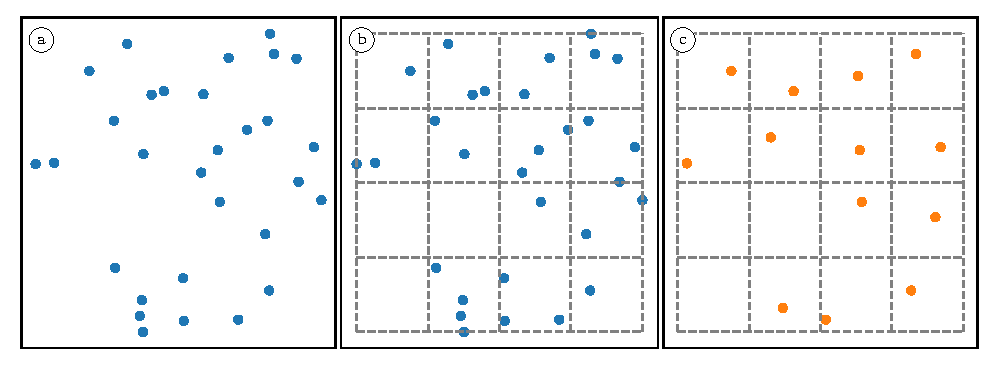
\includegraphics[width=\linewidth]{figs/block-median-sources-schematics.pdf}
    \caption{
        Block averaged sources.
        (a)~Given a set of observation points
        (b)~we divide the survey region on blocks of equal size and compute the
            median location of the observation points that fall inside each
            block.
        (c)~A source point is located beneath each block averaged coordinate.
            The number of point sources could be less or equal to the number of
            observation points. No source is located beneath unpopulated
            blocks.
    }
    \label{fig:block-median-sources}
\end{figure*}

The depth of the point sources can be chosen following different criteria.
Deep sources generate low frequencies, while shallow ones generate high
frequencies (cite).
The simplest option is to locate all sources at the same depth, which we will
call \emph{constant depth} in the future (see Fig.~\ref{fig:depth-types}(a)).
If the measurement were taken at significantly different altitudes, the
elevated computation points will be more distant to the sources than the lower
ones.
This may create problems on reproducing high frequencies on the elevated
points.

One possible solution is to locate each source bellow its corresponding
observation (or block averaged) point at a constant \emph{relative depth}
from it.
The depth of each source can be computed as the height of its corresponding
observation (or block averaged) point minus a depth parameter that assumes the
same value for all sources (see Fig.~\ref{fig:depth-types}(b)).
The sources won't be all at the same depth, but they will all be at the same
distance from their corresponding observation (or block averaged) point.

In case our survey presents heavily clustered data points on some areas, we may
want the sources bellow that region to be shallower in order to reproduce the
high frequencies measured by these clustered observation points.
We can propose a \emph{variable depth} approach: it locates each point source
according to the \emph{relative depth} and then subtracts a term proportional
to the mean distance to its $k$ nearest neighbour sources
(see Fig.~\ref{fig:depth-types}(c)).
So, the depth of the sources can be computed as follows:

\begin{equation}
    \begin{split}
        \textrm{depth} =
           &\textrm{data point height} - \textrm{relative depth} \\
           &- \textrm{depth factor} \cdot \textrm{mean distance}
    \end{split}
\end{equation}

\noindent where \emph{data point height} is the elevation of the corresponding
observation (or block averaged) point to the source, \emph{depth factor} and
\emph{relative depth} are parameters and \emph{mean distance} is the mean
distance to the $k$ nearest source neighbours.
This term will be smaller in case of clustered sources, making them shallower
than scattered and distant sources.

Similar approaches for setting sources at depths that depend
on the distance to their nearest neighbours were already proposed by
\citet{cordell1992, guspi2004, guspi2009}.

Worth mention that the two last approaches (the \emph{relative depth} and the
\emph{variable depth}) could not be applied to \emph{grid sources}.


\begin{figure*}
    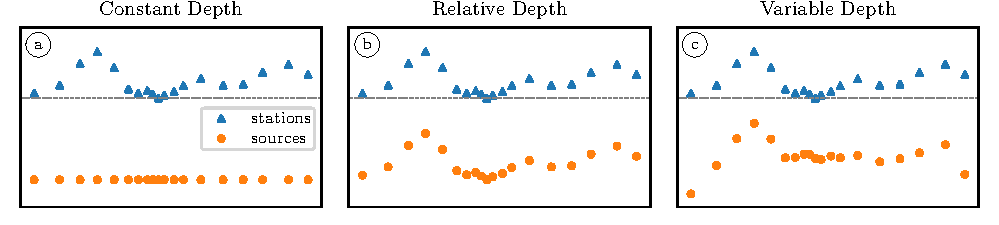
\includegraphics[width=\linewidth]{figs/depth_types.pdf}
    \caption{
        Depth types for locating point sources. We put one source beneath each
        observation point (station) using:
        (a)~a \emph{constant depth} where all sources are located at the same
           depth,
        (b)~a \emph{relative depth} where all sources are located at the same
           vertical distance from its corresponding observation point, and
        (c)~a \emph{variable depth} where the depth of the sources is
           proportional to the average distance to its neighbour sources.
           Notice how the clustered sources on (c) are relatively shallower
           than the
           other ones.
    }
    \label{fig:depth-types}
\end{figure*}

The combination of the three source layouts with the three strategies to define
the depth of the sources define seven different source distributions (see
Table~\ref{tab:source-distributions}).
The \emph{grid sources} is only compatible with the \emph{constant depth}
scheme.


\begin{table*}
    \centering
    \caption{
        Source distributions as combinations of source layouts and depth
        strategies.
    }
    \label{tab:source-distributions}
    \begin{tabular}{lccc}
        & Source bellow data & Block averaged sources & Grid sources \\ \hline
        Constant depth & $\checkmark$ & $\checkmark$ & $\checkmark$ \\
        Relative depth & $\checkmark$ & $\checkmark$ & $\times$     \\
        Variable depth & $\checkmark$ & $\checkmark$ & $\times$     \\
    \end{tabular}
\end{table*}


%%%%%%%%%%%%%%%%%%%%%%%%%%%%%%%%%%%%%%%%%%%%%%%%%%%%%%%%%%%%%%%%%%%%%%%%%%%%%%%

\section{Comparison of source distributions}

%Compare the accuracy of the predictions made by each source distribution.
%Need an objective way to compare them.
%Propose a synthetic gravity model made out of prisms of different sizes and
%density contrasts.
%Create a regular grid of observation points where the gravitational effect of
%the synthetic model will be computed.
%Call it the \emph{target grid}.
%Generate synthetic surveys above the same synthetic model and compute the
%gravitational effect of the model on each survey.
%Use each source distribution to predict values based on the ones obtained on
%each survey onto the same grid points of the \emph{target grid}.
%Score each interpolation by comparing the predicted values with the
%\emph{target grid}.
%Finally compare the accuracy of the predictions made by each source
%distribution.

Our goal is to to compare the performance of all source distributions from
Table~\ref{tab:source-distributions} when predicting harmonic field data using
the equivalent layer technique.
To do so we have created a synthetic model made out of prisms of different
shape and density contrasts.
The gravitational effect of this synthetic model have been computed on
a regular grid (\emph{target} grid) at a constant height and on two different
set of observation points that we will call \emph{synthetic surveys}: a ground
and an airborne survey.
The data from each synthetic survey is interpolated on the points of the
\emph{target} grid.
The interpolations are carried out using each source distribution and combining
different parameter values for each distribution.
Each prediction is then scored against the \emph{target} grid.
We can then quantitatively compare how accurate is each source distribution at
predicting unobserved data on each synthetic survey and quantify the
computational load needed to do it.

\subsection{Synthetic Model}

%Describe forward model made out of prisms.
%Show prisms model?

The synthetic model is made out of \NPrisms{} prisms distributed on a region of
\ModelEasting{}$\times$\ModelNorthing{} between \ModelDepth{} deep and the zero
height plane.
Density contrast of prisms range from \ModelMinDensity{} and
\ModelMaxDensity{}.
We created deep big and thin shallow prisms for creating gravity anomalies with
long and short wavelengths, respectively.

The vertical component of the gravity acceleration generated by the synthetic
model has been computed on a regular grid of
\TargetEastingSize{}$\times$\TargetNorthingSize{} points with a spacing of
\TargetSpacing{} located \TargetHeight{} above the zero height plane
(Fig.~\ref{fig:target-grid}).
We will refer to this grid as the \emph{target} grid in the future.

\begin{figure}
    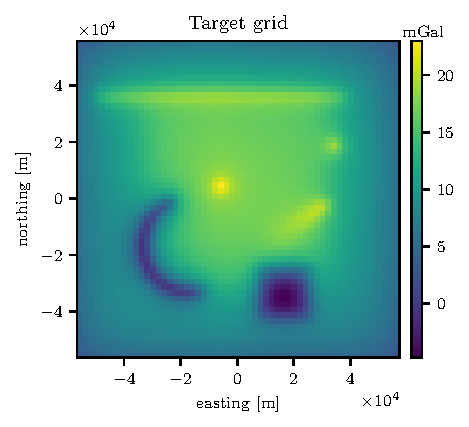
\includegraphics[width=\linewidth]{figs/target-grid.pdf}
    \caption{
        Target grid. Gravitational effect of synthetic model on a regular grid
        composed of \TargetEastingSize{}$\times$\TargetNorthingSize{} points
        with a spacing of \TargetSpacing{} located \TargetHeight{} above the
        zero height plane.
    }
    \label{fig:target-grid}
\end{figure}

\subsection{Synthetic Surveys}

In order to compare the predictive capabilities of each source distribution
under on different surveys, we created a ground and an airborne \emph{synthetic
surveys}.
For creating the synthetic ground survey we selected a portion of the Southern
Africa Gravity Data available through the
\href{https://www.ngdc.noaa.gov/mgg/gravity/gravity.html}{NOAA website}.
For the airborne survey we used a portion of the Great Britain Aeromagnetic
Survey acquired by Hunting Geology and Geophysics Ltd and Canadian Aeroservices
Ltd between 1955 and 1965 and made available by the
\href{https://www.bgs.ac.uk/products/geophysics/aeromagneticRegional.html}{
British Geological Survey (BGS)
}.

On both cases we selected only a portion of the survey and rescaled it to span
on an area of \SurveyEasting{}$\times$\SurveyNorthing{}.
The ground survey is composed by \GroundSurveyPoints{} observation points
distributed at heights ranging between \GroundSurveyMinHeight{} and
\GroundSurveyMaxHeight{} (Fig.~\ref{fig:synthetic-ground-survey}(a)).
While the airborne survey has \AirborneSurveyPoints{} points at heights between
\AirborneSurveyMinHeight{} and \AirborneSurveyMaxHeight{}.
(Fig.~\ref{fig:synthetic-ground-survey}(a)).

The vertical component of the gravity acceleration generated by the synthetic
model has been computed on both surveys.
Some Gaussian noise (with standard deviation of \SurveyNoise{}) has been added
to the effect of the synthetic model to simulate acquisition errors
(Figs.~\ref{fig:synthetic-ground-survey}(b)
and~\ref{fig:synthetic-airborne-survey}(b)).

\begin{figure}
    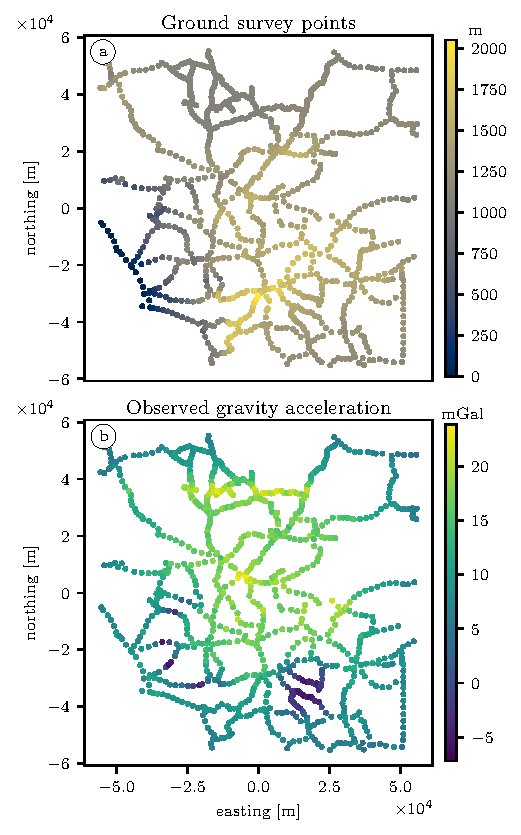
\includegraphics[width=\linewidth]{figs/ground-survey.pdf}
    \caption{
        Synthetic ground survey.
        (a)~Location of observation points. Altitude given in meters above the
            zero height plane.
        (b)~Vertical component of gravity acceleration generated by the
            synthetic model plus Gaussian noise on the ground survey
            observation points.
    }
    \label{fig:synthetic-ground-survey}
\end{figure}

\begin{figure}
    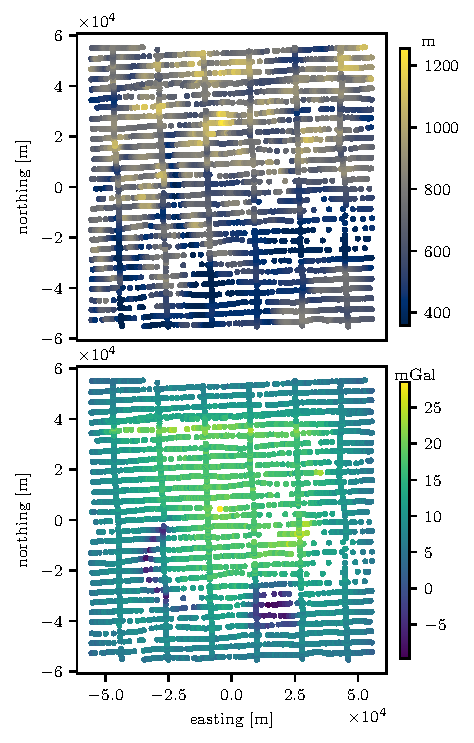
\includegraphics[width=\linewidth]{figs/airborne-survey.pdf}
    \caption{
        Synthetic airborne survey.
        (a)~Location of observation points. Altitude given in meters above the
            zero height plane.
        (b)~Vertical component of gravity acceleration generated by the
            synthetic model plus Gaussian noise on the airborne survey
            observation points.
        Based upon the Great Britain aeromagnetic data, with the permission of
        the British Geological Survey.
    }
    \label{fig:synthetic-airborne-survey}
\end{figure}

\subsection{Comparisons}

Each source distribution from Table~\ref{tab:source-distributions} needs
certain parameters in order to build the set of point sources.
The prediction capabilities of the source distribution depends on the choice of
these parameters.
For example, locating the sources beneath the data points at constant depth
needs the definition of the \emph{depth} parameter.
If the sources are set too close to the data points, the source distribution
it's very likely to overfit the data: the measured field will be recovered, but
the predictions on unobserved locations will be very inaccurate.
Another parameter that plays an important role on the predictive capabilities
of the sources is the damping parameter.
On real world scenarios, choosing the values of the parameters is a challenging
task: it's not easy to determine the accuracy of the predictions without
knowing the true value of the field on unobserved locations.
This problem can be solved through cross-validation.
When working with a synthetic model, the situation is different: we can compute
the true values of harmonic field generated by the synthetic model on any
point.
Therefore, interpolating the observed data on the same points of the
\emph{target} grid and then scoring the prediction against the true values of
the \emph{target} grid constitutes an objective way to measure the predictive
accuracy of the source distribution.

For each source distribution we proposed different values for each parameter
(including the damping) and combined them into several parameters sets.
For each parameter set we build the sources and fit their coefficients through
least-squares.
Then the sources are used to predict the field on the same points of the
\emph{target} grid and finally we compute the coefficient of determination
(R$^2$ score) between the prediction and the true values of the \emph{target}
grid.
We can therefore obtain the \emph{best prediction} generated by each source
distribution as the one that achieves the highest score.


\begin{table*}
    \centering
    \caption{
        Combination of parameters that produce the best prediction when
        gridding the synthetic ground survey with each source distribution.
        The score of each best prediction is also shown.
    }
    \label{tab:parameters-ground-survey}
    \begin{tabular}{l c c c}
        & \textbf{Sources bellow data} & \textbf{Block median sources}
        & \textbf{Grid sources} \\

        \textbf{Constant depth} & & & \\
        \hline
        Depth (m) & \BestGroundSourceBellowDataConstantDepthDepth
                   & \BestGroundBlockMedianSourcesConstantDepthDepth
                   & \BestGroundGridSourcesConstantDepthDepth \\
        Spacing (m) & -
                     & \BestGroundBlockMedianSourcesConstantDepthSpacing
                     & \BestGroundGridSourcesConstantDepthSpacing \\
        Pad & -
            & -
            & \BestGroundGridSourcesConstantDepthPad \\
        Damping & \BestGroundSourceBellowDataConstantDepthDamping
                & \BestGroundBlockMedianSourcesConstantDepthDamping
                & \BestGroundGridSourcesConstantDepthDamping \\
        \textbf{R$^2$ score}
                & \textbf{\BestGroundSourceBellowDataConstantDepthScore}
                & \textbf{\BestGroundBlockMedianSourcesConstantDepthScore}
                & \textbf{\BestGroundGridSourcesConstantDepthScore} \\

        & & & \\
        \textbf{Relative depth} & & & \\
        \cline{1-3}
        Depth (m) & \BestGroundSourceBellowDataRelativeDepthDepth
                   & \BestGroundBlockMedianSourcesRelativeDepthDepth
                   & \\
        Spacing (m) & -
                & \BestGroundBlockMedianSourcesRelativeDepthSpacing
                & \\
        Damping & \BestGroundSourceBellowDataRelativeDepthDamping
                & \BestGroundBlockMedianSourcesRelativeDepthDamping
                & \\
        \textbf{R$^2$ score}
                & \textbf{\BestGroundSourceBellowDataRelativeDepthScore}
                & \textbf{\BestGroundBlockMedianSourcesRelativeDepthScore}
                & \\

        & & & \\
        \textbf{Variable depth} & & & \\
        \cline{1-3}
        Depth (m) & \BestGroundSourceBellowDataVariableDepthDepth
                   & \BestGroundBlockMedianSourcesVariableDepthDepth
                   & \\
        Depth factor & \BestGroundSourceBellowDataVariableDepthDepthFactor
                     & \BestGroundBlockMedianSourcesVariableDepthDepthFactor
                     & \\
        K nearest & \BestGroundSourceBellowDataVariableDepthKNearest
                  & \BestGroundBlockMedianSourcesVariableDepthKNearest
                  & \\
        Spacing (m) & -
                     & \BestGroundBlockMedianSourcesVariableDepthSpacing
                     & \\
        Damping & \BestGroundSourceBellowDataVariableDepthDamping
                & \BestGroundBlockMedianSourcesVariableDepthDamping
                &  \\
        \textbf{R$^2$ score}
                & \textbf{\BestGroundSourceBellowDataVariableDepthScore}
                & \textbf{\BestGroundBlockMedianSourcesVariableDepthScore}
                & \\
    \end{tabular}
\end{table*}

\begin{table*}
    \centering
    \caption{
        Combination of parameters that produce the best prediction when
        gridding the synthetic airborne survey with each source distribution.
        The score of each best prediction is also shown.
    }
    \label{tab:parameters-ground-survey}
    \begin{tabular}{l c c c}
        & \textbf{Sources bellow data} & \textbf{Block median sources}
        & \textbf{Grid sources} \\

        \textbf{Constant depth} & & & \\
        \hline
        Depth (m) & \BestAirborneSourceBellowDataConstantDepthDepth
                   & \BestAirborneBlockMedianSourcesConstantDepthDepth
                   & \BestAirborneGridSourcesConstantDepthDepth \\
        Spacing (m) & -
                     & \BestAirborneBlockMedianSourcesConstantDepthSpacing
                     & \BestAirborneGridSourcesConstantDepthSpacing \\
        Pad & -
            & -
            & \BestAirborneGridSourcesConstantDepthPad \\
        Damping & \BestAirborneSourceBellowDataConstantDepthDamping
                & \BestAirborneBlockMedianSourcesConstantDepthDamping
                & \BestAirborneGridSourcesConstantDepthDamping \\
        R$^2$ score & \BestAirborneSourceBellowDataConstantDepthScore
                    & \BestAirborneBlockMedianSourcesConstantDepthScore
                    & \BestAirborneGridSourcesConstantDepthScore \\
        \textbf{R$^2$ score}
                & \textbf{\BestAirborneSourceBellowDataConstantDepthScore}
                & \textbf{\BestAirborneBlockMedianSourcesConstantDepthScore}
                & \textbf{\BestAirborneGridSourcesConstantDepthScore} \\

        & & & \\
        \textbf{Relative depth} & & & \\
        \cline{1-3}
        Depth (m) & \BestAirborneSourceBellowDataRelativeDepthDepth
                   & \BestAirborneBlockMedianSourcesRelativeDepthDepth
                   & \\
        Spacing (m) & -
                & \BestAirborneBlockMedianSourcesRelativeDepthSpacing
                & \\
        Damping & \BestAirborneSourceBellowDataRelativeDepthDamping
                & \BestAirborneBlockMedianSourcesRelativeDepthDamping
                & \\
        \textbf{R$^2$ score}
                & \textbf{\BestAirborneSourceBellowDataRelativeDepthScore}
                & \textbf{\BestAirborneBlockMedianSourcesRelativeDepthScore}
                & \\

        & & & \\
        \textbf{Variable depth} & & & \\
        \cline{1-3}
        Depth (m) & \BestAirborneSourceBellowDataVariableDepthDepth
                   & \BestAirborneBlockMedianSourcesVariableDepthDepth
                   & \\
        Depth factor & \BestAirborneSourceBellowDataVariableDepthDepthFactor
                     & \BestAirborneBlockMedianSourcesVariableDepthDepthFactor
                     & \\
        K nearest & \BestAirborneSourceBellowDataVariableDepthKNearest
                  & \BestAirborneBlockMedianSourcesVariableDepthKNearest
                  & \\
        Spacing (m) & -
                     & \BestAirborneBlockMedianSourcesVariableDepthSpacing
                     & \\
        Damping & \BestAirborneSourceBellowDataVariableDepthDamping
                & \BestAirborneBlockMedianSourcesVariableDepthDamping
                &  \\
        \textbf{R$^2$ score}
                & \textbf{\BestAirborneSourceBellowDataVariableDepthScore}
                & \textbf{\BestAirborneBlockMedianSourcesVariableDepthScore}
                & \\
    \end{tabular}
\end{table*}


%%%%%%%%%%%%%%%%%%%%%%%%%%%%%%%%%%%%%%%%%%%%%%%%%%%%%%%%%%%%%%%%%%%%%%%%%%%%%%%

\section{Discussion}

%%%%%%%%%%%%%%%%%%%%%%%%%%%%%%%%%%%%%%%%%%%%%%%%%%%%%%%%%%%%%%%%%%%%%%%%%%%%%%%

\section{Conclusions}

%%%%%%%%%%%%%%%%%%%%%%%%%%%%%%%%%%%%%%%%%%%%%%%%%%%%%%%%%%%%%%%%%%%%%%%%%%%%%%%

\section{Acknowledgements}

We are indebted to the developers and maintainers of the open-source software
without which this work would not have been possible.

The synthetic airborne survey was based upon the Great Britain aeromagnetic
data, reproduced with the permission of the British Geological Survey
$\textcopyright$UKRI\@.
All rights reserved.

%%%%%%%%%%%%%%%%%%%%%%%%%%%%%%%%%%%%%%%%%%%%%%%%%%%%%%%%%%%%%%%%%%%%%%%%%%%%%%%

\appendix

\section{Source distributions parameters}

\begin{table*}
    \centering
    \caption{
        Parameters used with each source distribution when gridding the
        synthetic ground survey.
    }
    \label{tab:parameters-ground-survey}
    \begin{tabular}{c | l l c c}
        \multicolumn{1}{c}{\textbf{Source layout}}
            & \multicolumn{1}{c}{\textbf{Depth type}}
            & \multicolumn{1}{c}{\textbf{Parameters}}
            & \multicolumn{1}{c}{\textbf{Values}}
            & \multicolumn{1}{c}{\textbf{Interval}} \\
        \hline

        \multirow{5}{*}{Source Bellow Data}
            & Constant Depth
                & Depth (km)
                & \GroundSourceBellowDataConstantDepthDepth
                & \GroundSourceBellowDataConstantDepthDepthInterval \\
            \cline{2-5}
            & Relative Depth
                & Depth (km)
                & \GroundSourceBellowDataRelativeDepthDepth
                & \GroundSourceBellowDataRelativeDepthDepthInterval \\
            \cline{2-5}
            & \multirow{3}{*}{Variable Depth}
                & Depth (km)
                & \GroundSourceBellowDataVariableDepthDepth
                & \GroundSourceBellowDataVariableDepthDepthInterval \\
            &
                & Depth factor
                & \GroundSourceBellowDataVariableDepthDepthFactor
                & \GroundSourceBellowDataVariableDepthDepthFactorInterval \\
            &
                & K nearest
                & \GroundSourceBellowDataVariableDepthKNearest
                & \GroundSourceBellowDataVariableDepthKNearestInterval \\
        \hline

        \multirow{8}{*}{Block median sources}
            & \multirow{2}{*}{Constant Depth}
                & Depth (km)
                & \GroundBlockMedianSourcesConstantDepthDepth
                & \GroundBlockMedianSourcesConstantDepthDepthInterval \\
            &
                & Spacing (km)
                & \GroundBlockMedianSourcesConstantDepthSpacing
                & \GroundBlockMedianSourcesConstantDepthSpacingInterval \\
            \cline{2-5}
            & \multirow{2}{*}{Relative Depth}
                & Depth (km)
                & \GroundBlockMedianSourcesRelativeDepthDepth
                & \GroundBlockMedianSourcesRelativeDepthDepthInterval \\
            &
                & Spacing (km)
                & \GroundBlockMedianSourcesRelativeDepthSpacing
                & \GroundBlockMedianSourcesRelativeDepthSpacingInterval \\
            \cline{2-5}
            & \multirow{4}{*}{Variable Depth}
                & Depth (km)
                & \GroundBlockMedianSourcesVariableDepthDepth
                & \GroundBlockMedianSourcesVariableDepthDepthInterval \\
            &
                & Depth factor
                & \GroundBlockMedianSourcesVariableDepthDepthFactor
                & \GroundBlockMedianSourcesVariableDepthDepthFactorInterval \\
            &
                & K nearest
                & \GroundBlockMedianSourcesVariableDepthKNearest
                & \GroundBlockMedianSourcesVariableDepthKNearestInterval \\
            &
                & Spacing (km)
                & \GroundBlockMedianSourcesVariableDepthSpacing
                & \GroundBlockMedianSourcesVariableDepthSpacingInterval \\
        \hline

        \multirow{3}{*}{Grid Sources}
            & \multirow{3}{*}{Constant Depth}
                & Depth (km)
                    & \GroundGridSourcesConstantDepthDepth
                    & \GroundGridSourcesConstantDepthDepthInterval \\
            &
                & Spacing (km)
                    & \GroundGridSourcesConstantDepthSpacing
                    & \GroundGridSourcesConstantDepthSpacingInterval \\
            &
                & Pad
                    & \GroundGridSourcesConstantDepthPad
                    & \GroundGridSourcesConstantDepthPadInterval \\
    \end{tabular}
\end{table*}

\begin{table*}
    \centering
    \caption{
        Parameters used with each source distribution when gridding the
        synthetic airborne survey.
    }
    \label{tab:parameters-airborne-survey}
    \begin{tabular}{l c c c}
        & \textbf{Sources bellow data} & \textbf{Block median sources}
        & \textbf{Grid sources} \\

        \textbf{Constant depth} & & & \\
        \hline
        Depth (km) & \AirborneSourceBellowDataConstantDepthDepth
                   & \AirborneBlockMedianSourcesConstantDepthDepth
                   & \AirborneGridSourcesConstantDepthDepth \\
        Spacing (km) & -
                     & \AirborneBlockMedianSourcesConstantDepthSpacing
                     & \AirborneGridSourcesConstantDepthSpacing \\
        Pad & -
            & -
            & \AirborneGridSourcesConstantDepthPad \\

        & & & \\
        \textbf{Relative depth} & & & \\
        \cline{1-3}
        Depth (km) & \AirborneSourceBellowDataRelativeDepthDepth
                   & \AirborneBlockMedianSourcesRelativeDepthDepth
                   & \\
        Spacing (km) & -
                     & \AirborneBlockMedianSourcesRelativeDepthSpacing
                     & \\

        & & & \\
        \textbf{Variable depth} & & & \\
        \cline{1-3}
        Depth (km) & \AirborneSourceBellowDataVariableDepthDepth
                   & \AirborneBlockMedianSourcesVariableDepthDepth
                   & \\
        Depth factor & \AirborneSourceBellowDataVariableDepthDepthFactor
                     & \AirborneBlockMedianSourcesVariableDepthDepthFactor
                     & \\
        K nearest & \AirborneSourceBellowDataVariableDepthKNearest
                  & \AirborneBlockMedianSourcesVariableDepthKNearest
                  & \\
        Spacing (km) & -
                     & \AirborneBlockMedianSourcesVariableDepthSpacing
                     & \\
    \end{tabular}
\end{table*}

%%%%%%%%%%%%%%%%%%%%%%%%%%%%%%%%%%%%%%%%%%%%%%%%%%%%%%%%%%%%%%%%%%%%%%%%%%%%%%%

\bibliographystyle{plainnat}
\bibliography{references}

\end{document}
